%===============================================================================
%===============================================================================
%
\clearpage
%
\subsection{Example-0101}
%
%===============================================================================
%
\subsubsection{Mathematical model}
%
We solve the following equation (both $2D$ and $3D$ domains are considered),
%
\begin{align}
    \nabla \cdot \boldsymbol{\sigma} (\boldsymbol{u}, t) = \boldsymbol{0} & &&\Omega = [0, 160] \times [0, 120] \times [0, 120], t \in [0, 5],
\end{align}
%
with time step size $\Delta_t = 1$ and $\boldsymbol{u} = [u_x,u_y]$ in $2D$ $\boldsymbol{u} = [u_x,u_y,u_z]$ in 3D. The boundary conditions in $2D$ are given by
%
\begin{align}
    u_x = u_y = 0 & &&x = y = 0, \\
		u_x = 16 & &&x = 160,
\end{align}
%
and in 3D by
\begin{align}
    u_x = u_y = u_z =0 & &&x = y = z =0, \\
		u_x = 16 & &&x = 160.
\end{align}
The material parameters are
\begin{align}
    E = & 10000\texttt{MPa}, \\
    \nu = & 0.3, \\
		\rho = & 5 \times 10^{-9}\texttt{tonne.mm$^3$}.
\end{align}
%
%===============================================================================
%
\subsubsection{Computational model}
%
\begin{itemize}
    \item{Commandline arguments are:}
        \subitem{float: length along x-direction}
        \subitem{float: length along y-direction}
        \subitem{float: length along z-direction (set to zero for 2D)}
        \subitem{integer: number of elements in x-direction}
        \subitem{integer: number of elements in y-direction}
        \subitem{integer: number of elements in z-direction (set to zero for 2D)}
        \subitem{integer: interpolation order (1: linear; 2: quadratic)}
        \subitem{integer: solver type (0: direct; 1: iterative)}
				\subitem{float: elastic modulus}
				\subitem{float: Poisson ratio}
				\subitem{float: displacement percentage load}
    \item{Commandline arguments for tests are:}
        \subitem{\ldots}
\end{itemize}
%
%===============================================================================
%
\subsubsection{Results}
%
\begin{figure}[h!]
    \centering 
    \includegraphics[width=\columnwidth]{examples/example-0101/doc/figures/analytical_solution.eps} 
    \caption{Results, analytical solution.}
    \label{example-0101-analytical-solution-fig}
\end{figure}
%
\begin{figure}[h!]
    \centering 
    \includegraphics[width=\columnwidth]{examples/example-0101/doc/figures/abaqus_reference.eps} 
    \caption{Results, Abaqus reference.}
    \label{example-0101-abaqus-reference-fig}
\end{figure}
%
\begin{figure}[h!]
    \centering 
    \includegraphics[width=\columnwidth]{examples/example-0101/doc/figures/iron_reference.eps} 
    \caption{Results, iron reference.}
    \label{example-0101-iron-reference-fig}
\end{figure}
%
\begin{figure}[h!]
    \centering 
    \includegraphics[width=\columnwidth]{examples/example-0101/doc/figures/current_run.eps} 
    \caption{Results, current run.}
    \label{example-0101-current-run-fig}
\end{figure}
%
%===============================================================================
%
\subsubsection{Validation}
%
CHeart rev.\ 6328, Abaqus 2017, analytical reference solution, whatever...
%
%===============================================================================
%===============================================================================
